\chapter{Design}
Now we will design how to implement what we have defined in the analysis chapter.

\section{Architecture}
\begin{figure}[h]
  \centering
  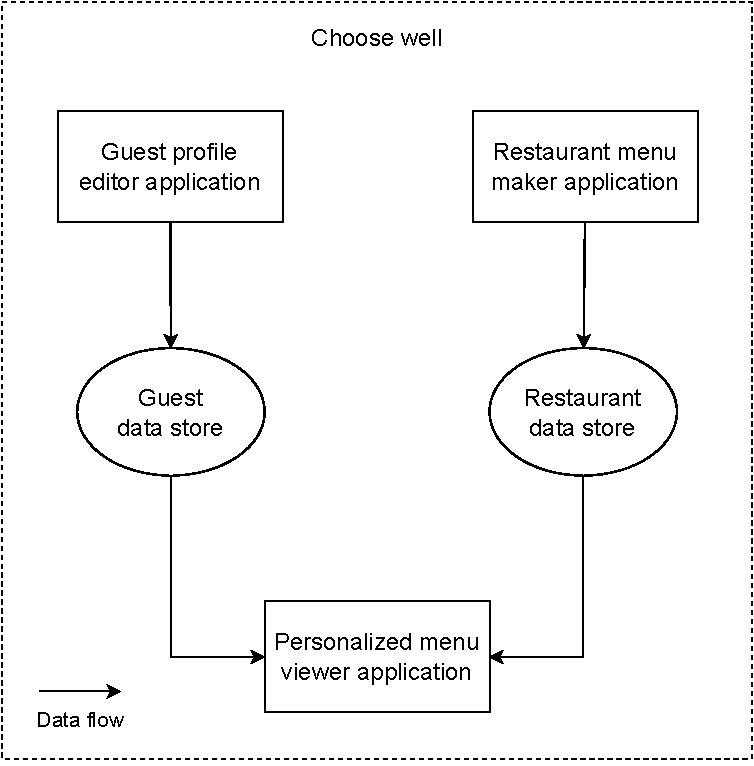
\includegraphics[width=0.62\linewidth]{master-thesis/img/architecture_data_flow.pdf}
  \caption{Application's data flow diagram}
\end{figure}

\section{Technological stack}
% popisat dostupne technologie, zoradit ich podla use case-u - responsive design, front-end frameworks, testovanie, dokumentácia (GitHub markdown) - v kazdom odstavci napisat preco som si danu technologiu vybral

\section{Wireframes}
\begin{figure}[h]
  \centering
  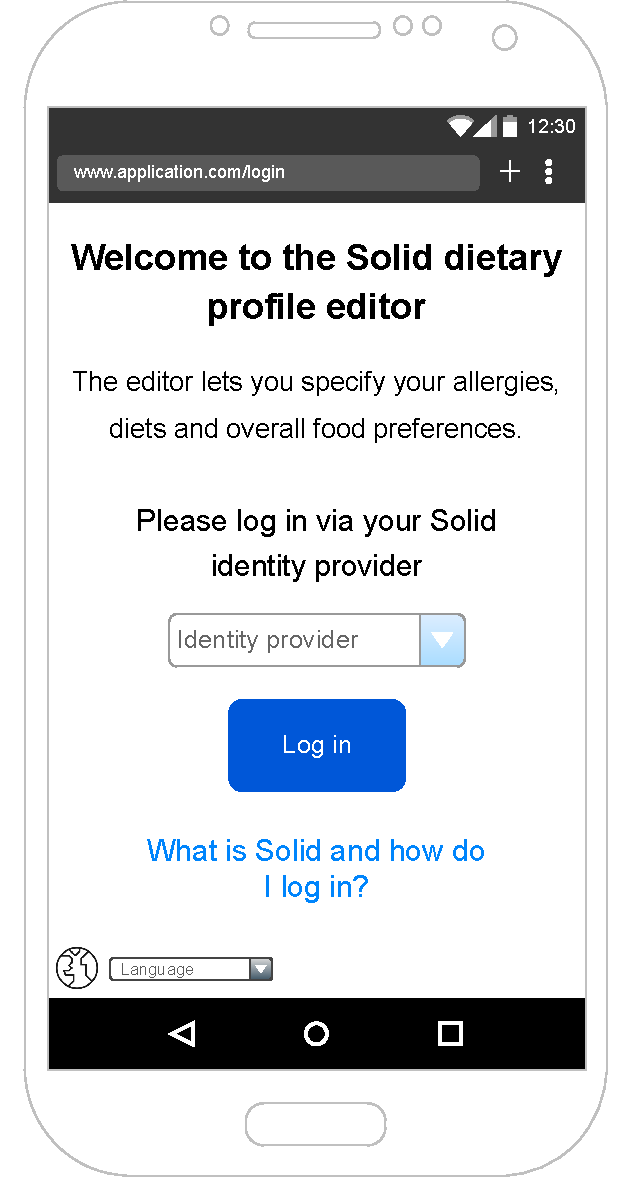
\includegraphics[width=0.62\linewidth]{master-thesis/img/wireframes/guest_profile_editor/login.pdf}
  \caption{Guest profile editor login screen}
\end{figure}

\begin{figure}[h]
  \centering
  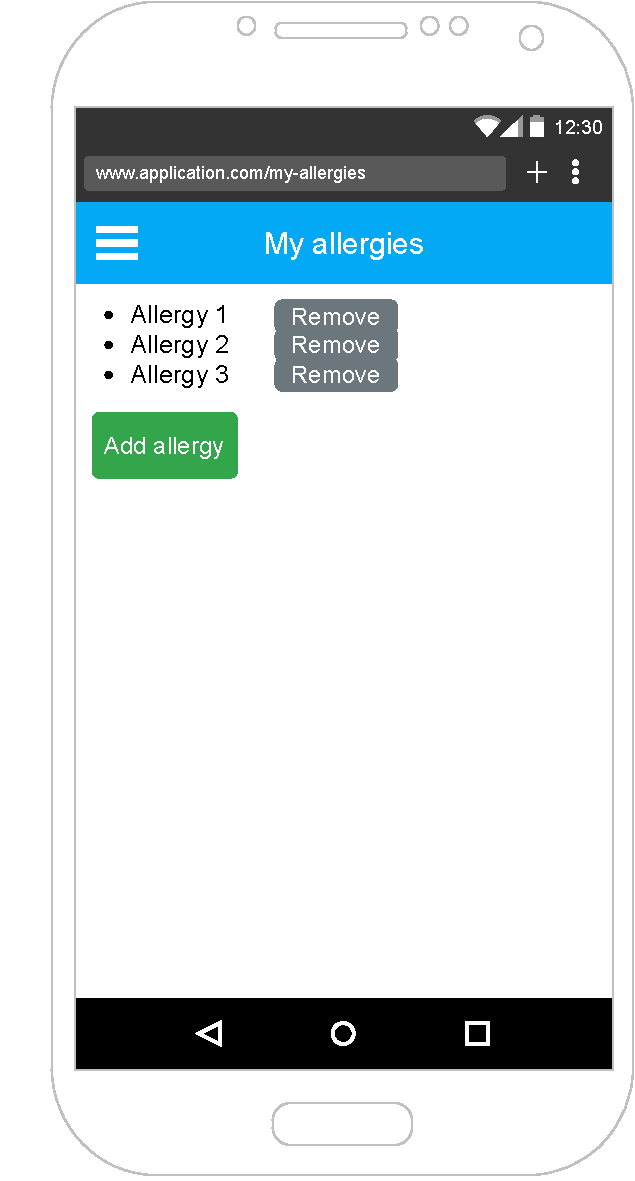
\includegraphics[width=0.62\linewidth]{master-thesis/img/wireframes/guest_profile_editor/my_allergies.pdf}
  \caption{Guest profile editor allergies screen}
\end{figure}

\begin{figure}[h]
  \centering
  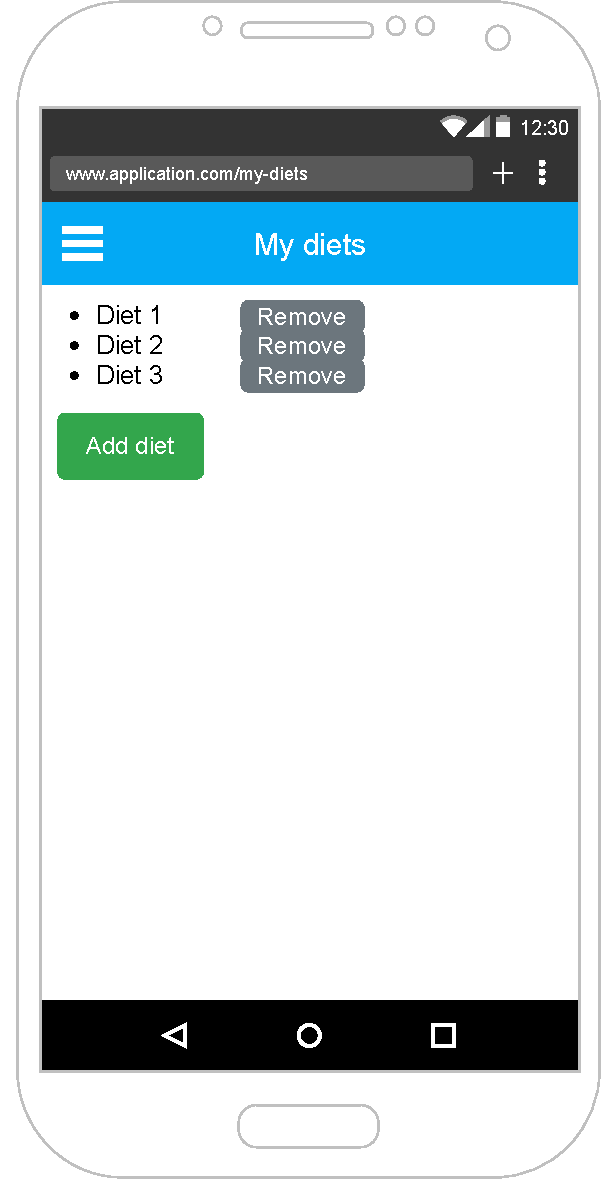
\includegraphics[width=0.62\linewidth]{master-thesis/img/wireframes/guest_profile_editor/my_diets.pdf}
  \caption{Guest profile editor diets screen}
\end{figure}

\begin{figure}[h]
  \centering
  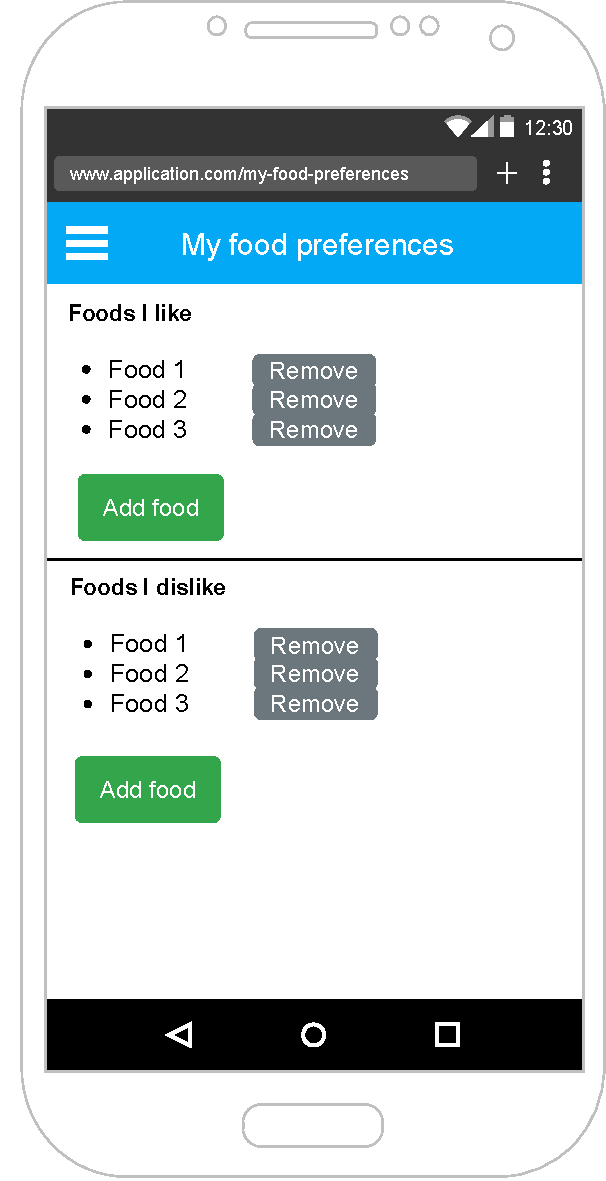
\includegraphics[width=0.62\linewidth]{master-thesis/img/wireframes/guest_profile_editor/my_food_preferences.pdf}
  \caption{Guest profile editor food preferences screen}
\end{figure}

\begin{figure}[h]
  \centering
  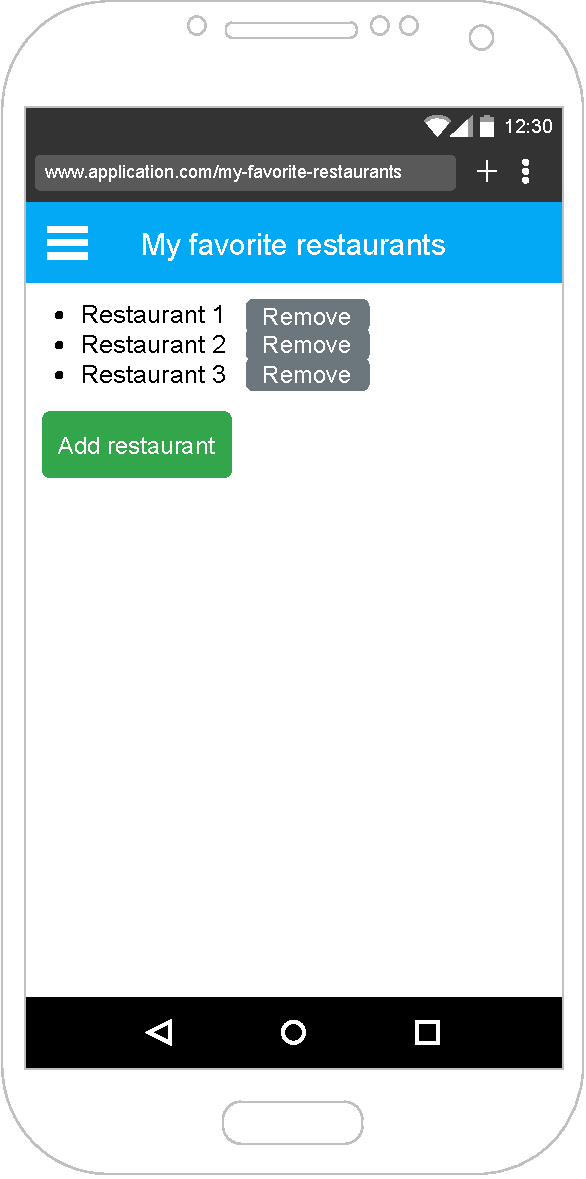
\includegraphics[width=0.62\linewidth]{master-thesis/img/wireframes/guest_profile_editor/my_favorite_restaurants.pdf}
  \caption{Guest profile editor favorite restaurants screen}
\end{figure}

\begin{figure}[h]
  \centering
  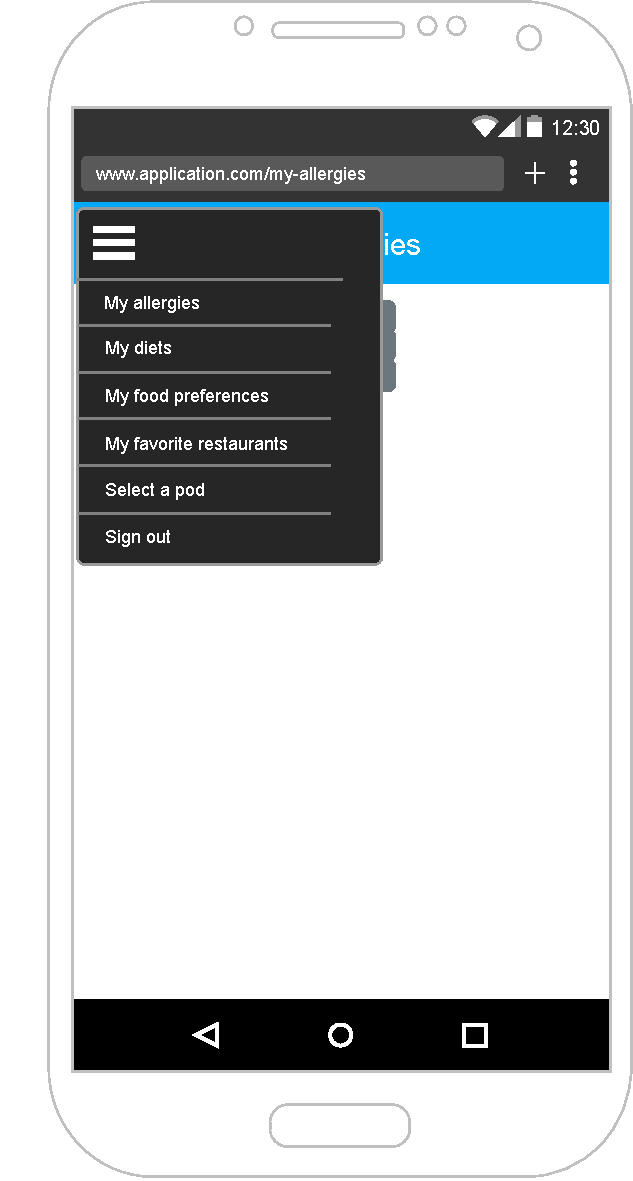
\includegraphics[width=0.62\linewidth]{master-thesis/img/wireframes/guest_profile_editor/menu_expanded.pdf}
  \caption{Guest profile editor screen with expanded menu}
\end{figure}

\listoftodos